% ============================================================
%  Capítulo 1 – Introdução
% ============================================================


\section{Cenário brasileiro de geração fotovoltaica}
\subsection{Dados atuais de geração}
\label{sec:cenario_brasileiro}

Segundo o Balanço Energético Nacional, divulgado em 2025 pela Empresa de
Pesquisa Energética (EPE), a energia solar fotovoltaica consolidou-se como a
fonte de maior crescimento da matriz brasileira nos últimos anos. Ao final de
2024, a capacidade instalada da fonte alcançou \SI{48,468}{\giga\watt},
representando uma expansão de \SI{28,1}{\percent} em relação ao ano anterior
\cite{EPE2025}. A geração de energia, consequentemente, também acompanhou esse ritmo, a produção solar fotovoltaica atingiu \SI{70,7}{\tera\watt\hour} em 2024, crescimento de
\SI{39,6}{\percent} sobre 2023 \cite{EPE2025}, conforme pode ser visto na Tabela \ref{tab:matriz_energetica}.

\begin{table}[!h]
    \centering
    \caption{Geração de energia elétrica e capacidade instalada no Brasil, 2023--2024.}
    \legend{Fonte: \citeonline{EPE2025}.}
\label{tab:matriz_energetica}
\begin{tabular}{lrrr}
\hline
\textbf{Fonte} & \textbf{2023} & \textbf{2024} & \textbf{$\Delta$\% 24/23} \\
\hline
\multicolumn{4}{l}{\textit{Geração (GWh)}} \\
\hline
Hidrelétrica          & 425.996 & 421.799 & $-$1,0\% \\
Gás Natural           &  38.589 &  47.792 & 23,9\%   \\
Eólica                &  95.801 & 107.654 & 12,4\%   \\
Biomassa              &  54.210 &  58.027 &  7,0\%   \\
Nuclear               &  14.504 &  15.767 &  8,7\%   \\
Carvão Vapor          &   8.770 &  10.247 & 16,8\%   \\
Derivados do Petróleo &   5.686 &   5.960 &  4,8\%   \\
\textbf{Solar Fotovoltaica} & \textbf{50.633} & \textbf{70.665} & \textbf{39,6\%} \\
Outras                &  13.932 &  13.425 & $-$3,6\% \\
\textbf{Geração Total}& \textbf{708.119} & \textbf{751.335} & \textbf{6,1\%} \\
\hline
\multicolumn{4}{l}{\textit{Capacidade Instalada (MW)}} \\
\hline
Hidrelétrica          & 109.922 & 109.922 &  0,0\%   \\
Térmica               &  47.515 &  46.439 & $-$2,3\% \\
Nuclear               &   1.990 &   1.990 &  0,0\%   \\
Eólica                &  28.682 &  29.550 &  3,0\%   \\
\textbf{Solar}        & \textbf{37.843} & \textbf{48.468} & \textbf{28,1\%} \\
\textbf{Capacidade Disponível} & \textbf{225.952} & \textbf{236.370} & \textbf{4,6\%} \\
\hline
\end{tabular}

\end{table}

Com efeito, ao caracterizar a inserção da fonte na matriz energética, é necessário distinguir
dois indicadores frequentemente confundidos. Em relação à matriz elétrica
nacional, na qual é contabilizada exclusivamente a geração de energia elétrica, a
solar respondeu por \SI{9,3}{\percent} do total em 2024 \cite{EPE2025}. Já em
relação à Oferta Interna de Energia (OIE), indicador mais amplo que abrange todas
as formas de energia consumidas no país, incluindo combustíveis para transporte e
processos industriais, a participação da fonte foi de \SI{2,2}{\percent}
\cite{EPE2025}. A diferença entre os dois percentuais é esperada e decorre da distinta abrangência de cada indicador e ao explicitá-la evita-se interpretações equivocadas sobre o real peso da fonte no sistema energético como um todo.

\begin{figure}[!h]
    \centering
    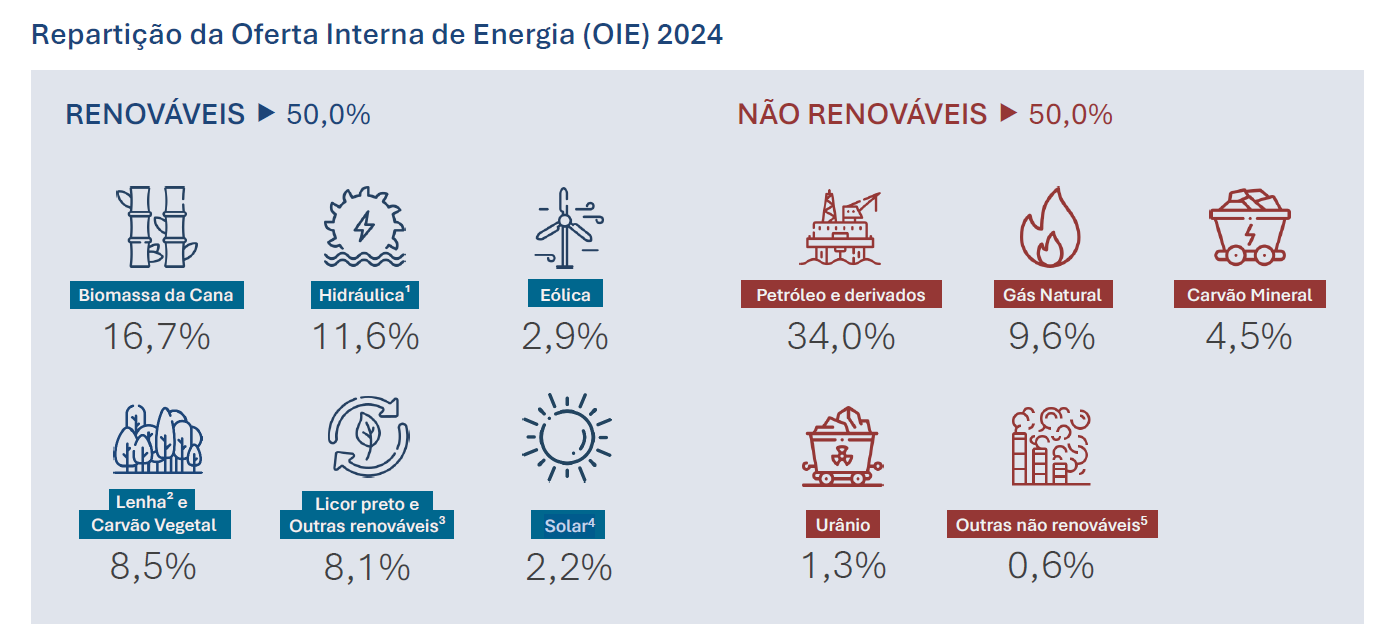
\includegraphics[width=0.65\linewidth]{figuras/introducao/dado_atuais/oie_2024.png}
    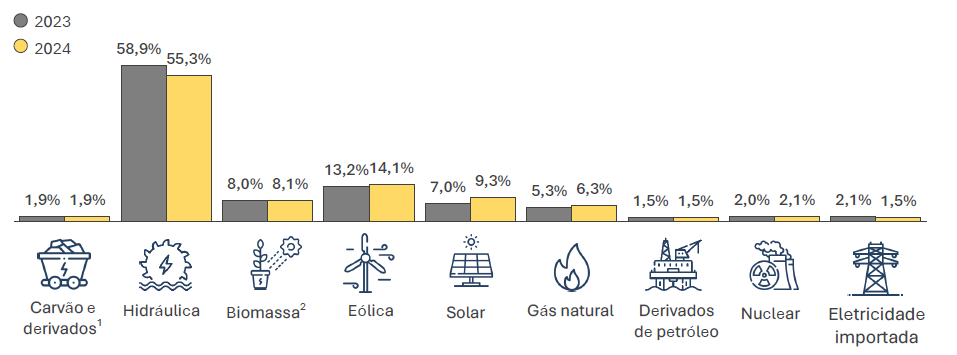
\includegraphics[width=0.65\linewidth]{figuras/introducao/dado_atuais/matriz_ele.png}
    \caption{De cima para abaixo: composição percentual da OIE para cada fonte de energia e composição percentual da matriz elétrica para cada fonte ambas para 2024.}
    \label{fig:placeholder}
    \legend{Fonte: \citeonline{EPE2025}.}
\end{figure}

Além disso, a energia fotovoltaica apresenta um elevado crescimento que torna-se evidente ao se analisar a série histórica. No âmbito da OIE, a participação da energia solar saltou de \SI{0,2}{\percent} em 2015 para \SI{2,2}{\percent} em 2024, configurando a fonte de maior crescimento
percentual no período \cite{EPE2025}. Esse avanço é impulsionado de forma expressiva pela micro e minigeração distribuída (MMGD), majoritariamente composta por sistemas fotovoltaicos, que já corresponde a cerca de \SI{5,6}{\percent} de toda a geração elétrica do país \cite{EPE2025}. Nesse sentido, os dados consolidados da evolução da participação das diferentes fontes na matriz elétrica e na OIE, são apresentados nas Figuras~\ref{fig:variacao-oie} e \ref{fig:matriz-eletrica}.

\newpage

\begin{figure}[!h]
    \centering
    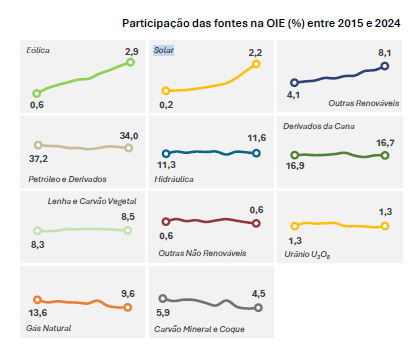
\includegraphics[width=0.5\linewidth]{figuras/introducao/dado_atuais/crescimento_fontes.png}
    \caption{Evolução temporal da participação de cada fonte de energia na OIE(\%) entre 2015 e 2024.}
    \legend{Fonte:\citeonline{EPE2025}}
    \label{fig:variacao-oie}
\end{figure}

\begin{figure}[!h]
    \centering
    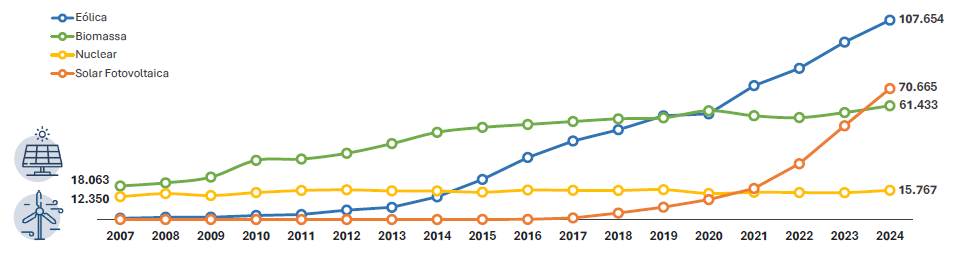
\includegraphics[width=0.9\linewidth]{figuras/introducao/dado_atuais/imagem_2026-05-31_204219085.png}
    \caption{Evolução da geração de energia elétrica por cada fonte.}
    \label{fig:matriz-eletrica}
    \legend{Fonte:\citeonline{EPE2025}}
\end{figure}

Dados mais recentes confirmam a continuidade dessa trajetória. Segundo a Associação Brasileira de Energia Solar Fotovoltaica, a capacidade fotovoltaica operacional no país superou \SI{70,3}{\giga\watt} em abril de 2026, considerando de forma agregada a geração centralizada e a distribuída \cite{absolar2026infografico}. Cabe observar que esse valor não é diretamente comparável aos \SI{48468}{\mega\watt} reportados pelo Balanço Energético Nacional, uma vez que se refere a uma data de corte posterior (abril de 2026, ante dezembro de 2024) e adota o critério metodológico do Ministério de Minas e Energia, que adiciona à capacidade instalada de cada fonte as parcelas associadas de micro e minigeração distribuída. Independentemente do critério, ambos os indicadores apontam para a mesma tendência de expansão acelerada.

Esse crescimento já produz efeitos sistêmicos relevantes. Em 26 de dezembro de 2025, a fonte solar atingiu o recorde de \SI{42552}{\mega\watt} de geração instantânea, equivalente a \SI{48,37}{\percent} da demanda nacional naquele momento; no mês de dezembro de 2025, respondeu por \SI{15,23}{\percent} de toda a oferta de energia elétrica do país \cite{absolar2026infografico}. Tal nível de penetração de uma fonte de caráter intermitente evidencia, contudo, os desafios operacionais associados à sua variabilidade, os quais serão retomados na Subseção~\ref{subsec:relevancia} como elemento central para a justificativa deste trabalho.

Dessa forma, os dados apresentados evidenciam que a energia fotovoltaica é uma fonte em ascensão, que em menos de uma década deixou de ser marginal para se tornar uma das protagonistas da expansão da matriz elétrica nacional. Esse desempenho expressivo, contudo, não decorre exclusivamente de incentivos regulatórios ou da redução de custos da tecnologia, mas encontra respaldo, sobretudo, nas condições físicas privilegiadas do território brasileiro para o aproveitamento da energia solar. Nesse sentido, para dimensionar adequadamente esse potencial e compreender o quanto dele ainda permanece inexplorado, faz-se necessário situar o Brasil no contexto internacional, comparando seus recursos e seu grau de aproveitamento com o de outros países.

\subsection{Comparação com outros países}
\label{subsec:comparacao_paises}

Apesar de expressiva, a expansão acelerada descrita na subseção anterior, ainda
representa uma fração modesta do potencial físico do território brasileiro. No entanto, para
dimensionar esse descompasso, é elucidativo confrontar o Brasil com duas das
maiores potências fotovoltaicas mundiais em capacidade instalada que é China e
Alemanha, distinguindo, primeiro, dois conceitos chaves: o
\emph{recurso solar disponível}, de natureza geográfica e climática, e o
\emph{grau de aproveitamento}, de natureza tecnológica,
econômica e regulatória. Os indicadores de recurso utilizados nesta comparação
provêm do estudo \textit{Global Photovoltaic Power Potential by Country}, produzido pelo
Banco Mundial em parceria com a Solargis \cite{WorldBank2020} e que padroniza,
para fins de comparabilidade entre países, a irradiação horizontal global
média (GHI, em \si{\kWh\per\square\metre\per\day}) como medida do potencial
teórico e a produtividade específica de uma usina de referência (PVOUT, em
\si{\kWh\per\kWp\day}) como medida do potencial prático.

\begin{figure}[!h]
    \centering
    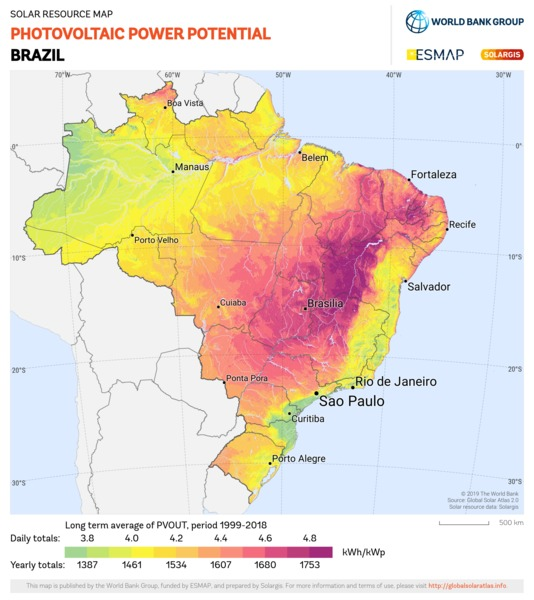
\includegraphics[width=0.3\linewidth]{figuras/introducao/comparacao/Brazil_PVOUT_mid-size-map_156x175mm-300dpi_v20191015.preview.jpg}
    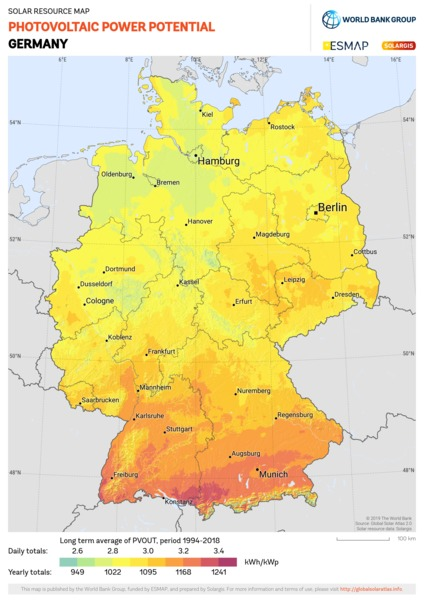
\includegraphics[width=0.3\linewidth]{figuras/introducao/comparacao/Germany_PVOUT_mid-size-map_156x220mm-300dpi_v20191205.preview.jpg}
    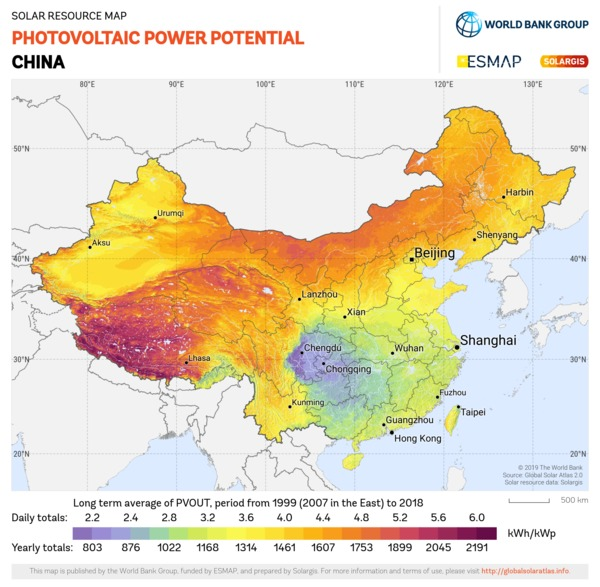
\includegraphics[width=0.3\linewidth]{figuras/introducao/comparacao/China_PVOUT_mid-size-map_156x152mm-300dpi_v20191015.preview.jpg}
    \caption{Mapas de produtividade fotovoltaica (PVOUT) do Brasil, Alemanha e China.}
    \label{fig:pvout-maps}
\end{figure}

A Alemanha é, historicamente, o país que pavimentou o mercado fotovoltaico
mundial, mas o faz a despeito de um recurso solar reconhecidamente escasso.
Segundo o estudo do Banco Mundial, o potencial teórico médio alemão é de apenas
\SI{2,978}{\kWh\per\square\metre\per\day} de GHI, ocupando a posição~197 no \textit{ranking}
mundial, ao passo que o Brasil registra \SI{5,276}{\kWh\per\square\metre\per\day},
ocupando a 89.\textsuperscript{a} posição \cite{WorldBank2020}. Em termos de
potencial prático, a produtividade média (PVOUT, nível~1) é de
\SI{2,961}{\kWh\per\kWp\per\day} na Alemanha contra
\SI{4,404}{\kWh\per\kWp\per\day} no Brasil \cite{WorldBank2020}. A diferença é
de tal ordem que o \textit{máximo} potencial prático observado em território
alemão (\SI{3,33}{\kWh\per\kWp\per\day}) é inferior ao \textit{mínimo}
registrado em qualquer ponto do território brasileiro
(\SI{3,75}{\kWh\per\kWp\per\day}) \cite{WorldBank2020}. Isto é, no
local menos ensolarado do Brasil é possível gerar mais eletricidade solar do
que no local mais ensolarado da Alemanha \cite{pereira2017atlas}. A esse maior
nível de irradiação soma-se uma vantagem qualitativa relevante para a operação
do sistema que é a baixa sazonalidade brasileira. Enquanto a razão entre o mês de
maior e o de menor produtividade (índice de sazonalidade) atinge $4{,}37$ na
Alemanha, no Brasil esse índice é de apenas $1{,}34$ \cite{WorldBank2020}, o que
se traduz em geração mais uniforme ao longo do ano e, portanto, em menor esforço
de balanço sazonal por parte do operador do sistema.

Apesar dessa inferioridade de recursos, a Alemanha mantém uma das maiores
bases instaladas do planeta, da ordem de \SI{117}{\giga\watt}, com adições
anuais médias próximas a \SI{19,6}{\giga\watt} \cite{BMWK2025}. Dessa forma, fica claro que o pioneirismo alemão decorreu não de condições naturais
favoráveis, mas de políticas de incentivo de longo prazo --- notadamente as
tarifas \textit{feed-in} ---, de maturidade industrial e de previsibilidade
regulatória. Essa constatação reforça que o aproveitamento da energia solar é
determinado tanto pelo recurso disponível quanto pelos arranjos
institucionais e tecnológicos que o viabilizam, dentre os quais se inclui a
capacidade de prever a geração com precisão, tema central deste trabalho.

Já a China apresenta um perfil intermediário no que tange ao recurso, mas é, em
larga margem, a líder absoluta em capacidade instalada. Seu potencial teórico
médio é de \SI{4,127}{\kWh\per\square\metre\day} de GHI (posição~161) e o
potencial prático médio, de \SI{3,883}{\kWh\per\kWp\day} de PVOUT
(posição~151) \cite{WorldBank2020}. Ambos os indicadores situam-se
significativamente abaixo dos valores brasileiros
(\SI{5,276}{\kWh\per\square\metre\per\day} e
\SI{4,404}{\kWh\per\kWp\day}, respectivamente), embora a heterogeneidade
territorial chinesa seja notável, o oeste do país, sobretudo o Deserto de Gobi e o Planalto Tibetano, exibem valores de PVOUT comparáveis aos melhores sítios brasileiros,
ao passo que as regiões orientais, mais populosas e industrializadas,
apresentam produtividade bastante inferior. Em relação a sazonalidade, o país apresenta um índice de $1{,}67$ \cite{WorldBank2020}, sendo superior à brasileira, porém, ainda que
mais favorável que a alemã.

No plano do aproveitamento, contudo, a assimetria se inverte de maneira
dramática. A China encerrou o período recente com capacidade fotovoltaica
instalada da ordem de \SI{1,23}{\tera\watt}, aproximadamente vinte vezes a
base instalada brasileira, além de ter um crescimento anual em torno de
\SI{33,2}{\percent} e com previsão de adição de \SIrange{180}{240}{\giga\watt}
ao longo de 2026 \cite{nea2026}. Apenas a expansão chinesa projetada para um
único ano supera, portanto, toda a capacidade fotovoltaica operacional no Brasil. O caso chinês evidencia uma faceta complementar à da Alemanha: trata-se de um país que não dispõe do melhor recurso solar, mas que, por meio de escala industrial, integração da cadeia produtiva e políticas de Estado, transformou a energia solar em pilar central de sua matriz elétrica.

A liderança chinesa, contudo, não se restringe à capacidade instalada em
território próprio, uma verz que o país consolidou-se também como o centro nevrálgico da
cadeia produtiva global de equipamentos fotovoltaicos. Em 2024, a China foi
responsável por \SI{93,2}{\percent} da produção mundial de polissilício,
\SI{96,6}{\percent} das lâminas (\textit{wafers}), \SI{92,3}{\percent} das
células fotovoltaicas e \SI{86,4}{\percent} dos módulos \cite{Davidson2026}.
Essa concentração, somada à escala de produção, pressionou os preços dos módulos
a mínimos históricos --- frequentemente abaixo de \SI{1}{RMB\per\watt} ---,
tornando-os economicamente inviáveis para fabricantes de outras regiões
\cite{Davidson2026}. Tal domínio reforça a constatação anterior de que o avanço
chinês na geração apoia-se em uma posição dominante sobre toda a cadeia de valor,
desde a matéria-prima até o produto final, o que situa o país não apenas como o
maior gerador, mas como o principal fornecedor mundial da tecnologia. Cabe
ressaltar, ainda, o vigor da expansão recente: somente em 2025 a China adicionou
cerca de \SI{315}{\giga\watt} de capacidade fotovoltaica \cite{PVMagazine2026},
montante que, isoladamente, supera várias vezes toda a capacidade instalada
acumulada pelo Brasil até o presente.

A Tabela~\ref{tab:comparacao_paises} consolida os principais indicadores
discutidos, contrastando o recurso solar disponível com o grau de
aproveitamento em cada país.

\begin{table}[htbp]
\centering
\caption{Comparativo de potencial solar, capacidade instalada e crescimento:
Brasil, China e Alemanha.}
\label{tab:comparacao_paises}
\begin{tabular}{lrrr}
\hline
\textbf{Indicador} & \textbf{Brasil} & \textbf{China} & \textbf{Alemanha} \\
\hline
\multicolumn{4}{l}{\textit{Recurso solar (longo prazo)\textsuperscript{a}}} \\
\hline
Potencial teórico (kWh/m\textsuperscript{2}/dia) & 5,276 & 4,127 & 2,978 \\
\quad \textit{posição no ranking mundial}                & 89.\textsuperscript{o} & 161.\textsuperscript{o} & 197.\textsuperscript{o} \\
Potencial prático (kWh/kWp/dia)                & 4,404 & 3,883 & 2,961 \\
\quad \textit{posição no ranking mundial}                & 84.\textsuperscript{o} & 151.\textsuperscript{o} & 197.\textsuperscript{o} \\
Sazonalidade ($-$)                             & 1,34 & 1,67 & 4,37 \\
Área equivalente                      & 0,03\% & 0,46\% & 2,95\% \\
\hline
\multicolumn{4}{l}{\textit{Aproveitamento (dados recentes)\textsuperscript{b}}} \\
\hline
Capacidade instalada                                     & $\approx$70,3 GW & $\approx$1.230 GW & $\approx$117 GW \\
Adição/crescimento recente                               & +28,1\%/ano & +315 GW (2025) & +19,6 GW/ano \\
\hline
\end{tabular}
\legend{\textsuperscript{a}~Fonte: \citeonline{WorldBank2020}, referente ao
estudo \textit{Global Photovoltaic Power Potential by Country} (dados de longo
prazo, 2020). \\
\textsuperscript{b}~Capacidade do Brasil em abril de 2026
\cite{absolar2026infografico}; capacidade e crescimento da China
\cite{nea2026,PVMagazine2026}; capacidade e crescimento da Alemanha
\cite{BMWK2025}. O crescimento do Brasil refere-se à expansão da capacidade
instalada em 2024 sobre 2023 \cite{EPE2025}.}
\end{table}

A confrontação com Alemanha e China revela um quadro paradoxal. O Brasil reúne,
simultaneamente, um recurso solar superior ao desses dois países com uma maior
irradiação média e, sobretudo, uma menor sazonalidade, além de um grau de
aproveitamento ainda incipiente quando medido em termos relativos, isto é, a área
equivalente necessária para suprir todo o consumo elétrico nacional com geração
fotovoltaica é estimada em apenas \SI{0,03}{\percent} do território, contra
\SI{0,46}{\percent} da China e \SI{2,95}{\percent} da Alemanha
\cite{WorldBank2020}, um indicador que sintetiza a folga existente entre
potencial e exploração. Fica evidente, assim, que o gargalo brasileiro não
reside no recurso natural, mas na capacidade de integrar de forma eficiente e
confiável uma fonte de caráter intermitente a um sistema elétrico de dimensões
continentais. É precisamente nesse ponto que se insere a contribuição deste
trabalho uma previsão acurada da geração fotovoltaica constitui um elemento
habilitador para que o vasto potencial brasileiro --- particularmente o da
região Nordeste, abordado na subseção seguinte --- seja convertido em geração
efetiva e despachável, mitigando os efeitos de sua variabilidade sobre a
operação do sistema.

\subsection{Grande potencial ainda não totalmente aproveitado no Nordeste}
\label{subsec:potencial_nordeste}

A vantagem brasileira evidenciada na comparação internacional não se distribui
de modo homogêneo pelo território. Conforme atestado pela segunda edição do
\textit{Atlas Brasileiro de Energia Solar}, elaborado pelo Laboratório de
Modelagem e Estudos de Recursos Renováveis de Energia (LABREN) do Instituto
Nacional de Pesquisas Espaciais (INPE) a partir do modelo de transferência
radiativa BRASIL-SR, a região Nordeste concentra os maiores níveis de
irradiação solar do país \cite{Pereira2017}. Os mapas de irradiação global
horizontal (GHI) ali apresentados situam o semiárido nordestino, em especial o
interior da Bahia e o vale do São Francisco, na faixa de maior incidência da
escala nacional, com totais diários médios anuais que se aproximam do limite
superior observado no território, da ordem de \SI{6,5}{\kWh\per\square\metre\per\day}
\cite{Pereira2017}. Em termos de potencial prático, os dados do estudo
\textit{Global Photovoltaic Power Potential by Country} corroboram essa
constatação, enquanto a mediana brasileira de PVOUT é de
\SI{4,42}{\kWh\per\kWp\day}, o valor máximo registrado no país alcança
\SI{4,92}{\kWh\per\kWp\day}, patamar associado justamente às áreas do
Nordeste \cite{WorldBank2020}.

A esse recurso de elevada magnitude soma-se uma característica de grande
relevância para a operação de sistemas fotovoltaicos que é a baixa variabilidade
sazonal. O regime de irradiação do semiárido é marcado por reduzida cobertura
de nuvens e pequena oscilação ao longo do ano, o que confere à região um índice
de sazonalidade inferior ao da média nacional \cite{Pereira2017,WorldBank2020}.
Tal estabilidade é tecnicamente desejável, pois implica geração mais uniforme
entre as estações e, consequentemente, maior previsibilidade da produção
energética, um atributo que, como se discutirá adiante, é determinante para a
integração da fonte ao sistema elétrico.

Esse conjunto de fatores físicos explica a forte concentração da geração
centralizada na região. De acordo com o levantamento mais recente da
Associação Brasileira de Energia Solar Fotovoltaica, entre os estados com maior
capacidade fotovoltaica centralizada outorgada figuram, logo após Minas Gerais,
a Bahia (\SI{20293,1}{\mega\watt}), o Piauí (\SI{17388,1}{\mega\watt}), o Ceará
(\SI{14503,5}{\mega\watt}), o Rio Grande do Norte (\SI{9383,1}{\mega\watt}), a
Paraíba (\SI{4087,2}{\mega\watt}) e Pernambuco (\SI{3812,1}{\mega\watt})
\cite{absolar2026infografico}. Considerados em conjunto, os estados nordestinos
respondem pela maior parcela da capacidade centralizada do país, refletindo a
preferência dos empreendimentos de grande porte por sítios de elevada
produtividade.

Subsiste, contudo, um descompasso expressivo entre o recurso disponível e o
montante efetivamente convertido em geração, descompasso esse que tende a se
agravar à medida que a capacidade instalada cresce mais rapidamente do que a
infraestrutura de transmissão e os mecanismos de gestão da rede. Um indício
concreto desse limite operacional já em curso é o aumento dos cortes de geração
(\textit{curtailment}) impostos às usinas solares: segundo o Operador Nacional
do Sistema, as restrições de geração em usinas fotovoltaicas cresceram de forma
acentuada nos últimos anos, alcançando, em 2025, montante equivalente a cerca
de \SI{20,7}{\percent} da geração \cite{absolar2026infografico}. Em outras
palavras, parcela relevante da energia que a região é fisicamente capaz de
produzir deixa de ser injetada na rede, o que evidencia que o gargalo brasileiro
--- e nordestino em particular --- reside não na disponibilidade do recurso, mas
na capacidade de integrá-lo de forma confiável a um sistema elétrico de
dimensões continentais.

Para dimensionar a ordem de grandeza desse potencial, é elucidativo um exercício
de estimativa. Adotando-se a produtividade específica máxima reportada para o
território nacional pelo \textit{Global Photovoltaic Power Potential by Country},
de \SI{4,92}{\kWh\per\kWp\per\day} --- equivalente a aproximadamente
\SI{1796}{\kWh\per\kWp} ao ano \cite{WorldBank2020} --- e uma densidade de
potência instalada característica de usinas de grande porte com módulos fixos de
silício cristalino, situada na faixa de \SIrange{60}{75}{\watt\peak\per\square\metre}
quando contabilizado o espaçamento entre fileiras\footnote{A densidade de
potência considera a área total ocupada pela usina, incluindo o espaçamento
entre fileiras de módulos necessário para evitar sombreamento mútuo, e não
apenas a área ativa dos painéis. A produtividade específica refere-se a sistemas
fixos com módulos monofaciais de silício cristalino e inclinação ótima, conforme
a metodologia adotada em \citeonline{WorldBank2020}. Trata-se de uma estimativa
de ordem de grandeza, que não incorpora restrições de uso do solo, áreas de
preservação, disponibilidade hídrica ou limitações da infraestrutura de
transmissão.}, é possível estimar o potencial de geração associado à ocupação de
diferentes frações da área da região Nordeste, cuja extensão territorial é de
cerca de \SI{1,55e6}{\square\kilo\metre}.

Os resultados, sintetizados na Tabela~\ref{tab:potencial_nordeste}, evidenciam a
magnitude do recurso. A ocupação de apenas \SI{1}{\percent} do território
nordestino seria suficiente para gerar entre \num{1675} e \SI{2093}{\tera\watt\hour}
por ano, montante equivalente a cerca de \numrange{2,2}{2,8} vezes toda a energia
elétrica gerada no Brasil em 2024 (\SI{751}{\tera\watt\hour}). Caso a fração
considerada fosse de \SI{5}{\percent}, a geração teórica superaria em mais de dez
vezes a produção nacional atual. Tais valores não representam, evidentemente,
metas de implantação --- são fisicamente irrealizáveis em sua totalidade ---, mas
explicitam a folga existente entre o recurso disponível e seu aproveitamento, bem
como reforçam que a limitação ao avanço da fonte não é de natureza física, e sim
operacional e sistêmica.

\begin{table}[!h]
\centering
\caption{Estimativa de ordem de grandeza do potencial de geração fotovoltaica do
Nordeste para diferentes frações de ocupação territorial.}
\legend{Fonte: elaborado pelo autor a partir de \citeonline{WorldBank2020} e
\label{tab:potencial_nordeste}
\begin{tabular}{lrrr}
\hline
\textbf{Fração da área} & \textbf{Densidade} & \textbf{Capacidade} & \textbf{Geração anual} \\
\textbf{do Nordeste}    & \textbf{(W$_p$/m\textsuperscript{2})} & \textbf{(GW$_p$)} & \textbf{(TWh/ano)} \\
\hline
\multirow{2}{*}{1\%} & 60 &   933 & 1.675 \\
                     & 75 & 1.166 & 2.093 \\
\hline
\multirow{2}{*}{5\%} & 60 & 4.663 &  8.374 \\
                     & 75 & 5.829 & 10.467 \\
\hline
\end{tabular}
\end{table}
\citeonline{EPE2025}. Premissas: PVOUT de \SI{4,92}{\kWh\per\kWp\per\day}
($\approx$\SI{1796}{\kWh\per\kWp\per\year}); área do Nordeste de
\SI{1,55e6}{\square\kilo\metre}. Comparação: geração elétrica total do Brasil em
2024 $=$ \SI{751}{\tera\watt\hour} \cite{EPE2025}.}

\subsection{Empecilhos para aproveitar o potencial}
\label{subsec:empecilhos}

A análise das subseções anteriores deixa claro que o gargalo brasileiro para a
expansão da geração fotovoltaica não reside na disponibilidade do recurso solar,
mas em um conjunto de fatores de natureza operacional, técnica e
institucional. A literatura especializada converge ao apontar que a distância
entre o potencial físico e o efetivamente convertido em geração decorre de
barreiras que extrapolam a dimensão econômica usualmente enfatizada
\cite{Fratea2017,Queiroz2020}. Dessa forma, discutem-se, nesta subseção, três desses
empecilhos: a capacidade limitada da infraestrutura de transmissão, a
escassez de mão de obra técnica qualificada e o ambiente tributário-regulatório, selecionados por sua relevância recorrente na literatura e por sua conexão
direta com a justificativa deste trabalho.

Entre as barreiras de caráter técnico, a insuficiência da rede de transmissão é
reiteradamente apontada como a mais crítica para a viabilização de
empreendimentos de grande porte. Nesse cenário, um estudo conduzido com agentes do setor
elétrico do estado de Minas Gerais, \citeonline{Fratea2017} identificaram, por
meio do método~Q, que a percepção de que ``a rede de transmissão de eletricidade
não dispõe de capacidade para escoar a eletricidade solar que a geração
fotovoltaica pode produzir'' figura entre as barreiras estatisticamente mais
significativas e mais bem ranqueadas pelos \emph{stakeholders}. Para esse grupo,
o gargalo de transmissão é considerado mais determinante do que o próprio preço
ofertado nos leilões, sob o argumento de que a elevada irradiação de um sítio é
condição necessária, mas não suficiente, à viabilidade do projeto: ``usinas
solares instaladas em locais de alta radiação não têm valor algum se não houver
meio de escoar a energia'' \cite{Fratea2017}. O mesmo estudo registra um caso
emblemático em que uma usina projetada para gerar \SI{2,78}{\mega\watt} de pico
estava limitada por uma capacidade local de rede de apenas \SI{1,25}{\mega\watt}
\cite{Fratea2017}, ilustrando o descasamento entre a capacidade de geração e a de
escoamento.

Esse diagnóstico, formulado em 2017, materializa-se hoje em um indicador
concreto e crescente que é o corte de geração (\textit{curtailment}). Conforme já
mencionado na Subseção~\ref{subsec:potencial_nordeste}, as restrições de geração
impostas às usinas fotovoltaicas pelo Operador Nacional do Sistema alcançaram,
em 2025, montante equivalente a cerca de \SI{20,7}{\percent} da geração total
\cite{absolar2026infografico}. Em outras palavras, a barreira de transmissão
deixou de ser uma projeção teórica e tornou-se uma perda mensurável de energia
já geráveis, agravada pelo fato de a expansão da capacidade instalada ocorrer em
ritmo superior ao da ampliação das linhas de transmissão.

Um segundo empecilho, de natureza estrutural, é a carência de profissionais
tecnicamente capacitados para sustentar o ciclo de vida dos sistemas
fotovoltaicos. \citeonline{Fratea2017} relatam forte concordância entre os
agentes do setor com a afirmação de que ``a ausência de mão de obra
especializada prejudica o desenvolvimento de usinas solares'', justificada pela
necessidade de capacidade técnica especializada ``desde a concepção do projeto
até a instalação, operação e manutenção''. Um dos entrevistados adverte, de
forma incisiva, que a falta de mão de obra qualificada ``resultará em falhas
operacionais, o que poderia favorecer tecnologias mais consolidadas, como a
hidreletricidade'' \cite{Fratea2017} --- observação particularmente relevante
para este trabalho, na medida em que falhas operacionais e a baixa qualidade
da operação comprometem diretamente a previsibilidade e a confiabilidade da
geração.

Essa lacuna é igualmente apontada como uma das limitações intrínsecas da fonte
em revisões da literatura, que listam a ``falta de especialistas para
manutenção, inspeção, reparo e avaliação'' entre as principais barreiras ao
aproveitamento da energia solar \cite{Queiroz2020}. A dimensão do
empecilho fica evidente no contraste internacional: na Alemanha, em 2013, o
setor de energias renováveis já empregava mais de \num{370000} trabalhadores em
empregos diretos, número que ultrapassava \num{1,5} milhão quando consideradas as
atividades de pesquisa, desenvolvimento, treinamento e educação associadas
\cite{Queiroz2020}. Cabe registrar, contudo, uma ressalva: parte da literatura
argumenta que essa barreira é mitigável no médio prazo, dada a existência, em
regiões de elevado potencial, de instituições de ensino técnico e superior
capazes de formar a mão de obra necessária localmente \cite{Fratea2017}. Trata-se,
portanto, de um empecilho real, porém endereçável por meio de políticas de
qualificação profissional.

O terceiro grupo de empecilhos relaciona-se ao arcabouço tributário e
regulatório. Por um lado, o marco regulatório foi historicamente o principal
catalisador da expansão da fonte no país: a Resolução Normativa
n.\textsuperscript{o}~482/2012 da Agência Nacional de Energia Elétrica (ANEEL),
ao regulamentar o sistema de compensação de energia da micro e minigeração
distribuída, e os leilões específicos para usinas fotovoltaicas conduzidos pelo
governo federal foram determinantes para o crescimento observado
\cite{Urbanetz2018}. Por outro lado, a própria literatura reconhece que a
maturidade de mercados consolidados decorreu de instrumentos de incentivo de
longo prazo --- como as tarifas \textit{feed-in} adotadas na Alemanha e na
Espanha --- combinados a reduções e isenções tributárias sobre equipamentos e
sobre o lucro das empresas atuantes no setor \cite{Fratea2017,Queiroz2020}.

No caso brasileiro, a carga tributária e os custos de capital ainda elevados
contribuem para que o custo de implantação supere o de países de referência: em
2013, enquanto o custo de instalação na Alemanha era da ordem de
\SI{1684}{\text{\euro}\per\kWp}, no Brasil situava-se entre \num{2000} e
\SI{3000}{\text{\euro}\per\kWp}, isto é, praticamente o dobro \cite{Queiroz2020}.
Soma-se a isso a instabilidade do ambiente regulatório, frequentemente
identificada como barreira política, uma vez que a incerteza quanto à
manutenção das regras de incentivo eleva o risco percebido pelo investidor e
inibe o aporte de capital no setor \cite{Queiroz2020,Fratea2017}. Análises
quantitativas das barreiras à expansão da fonte no país sugerem, inclusive, que
as barreiras de natureza política e de conhecimento exercem influência superior
à das barreiras estritamente financeiras, ambientais e sociais
\cite{Queiroz2020}, o que reforça a centralidade dos arranjos institucionais ---
e não apenas do custo da tecnologia --- na explicação do aproveitamento ainda
incipiente do potencial brasileiro.

Em suma, os três empecilhos discutidos compartilham uma característica comum:
nenhum deles decorre de limitações do recurso solar, e todos se intensificam à
medida que a participação de uma fonte intermitente cresce na matriz elétrica.
A capacidade de transmissão, a disponibilidade de mão de obra e a estabilidade
regulatória condicionam o quanto do potencial físico pode ser efetivamente
convertido em geração confiável e despachável. É nesse contexto que se insere a
contribuição deste trabalho, conforme se detalha na subseção seguinte.

\subsection{Conexão com o trabalho apresentado e sua relevância}
\label{subsec:relevancia}

As subseções anteriores estabeleceram dois fatos centrais, primeiro, o Brasil dispõe de um
recurso solar excepcional, particularmente no Nordeste, e, segundo, o aproveitamento desse
recurso não é limitado por sua disponibilidade física, mas por barreiras de
natureza operacional, técnica e institucional. Resta, portanto, articular de que
modo um modelo de previsão de geração contribui para a superação dessas barreiras, 
articulação que constitui a justificativa central deste trabalho.

Nesse sentido, o ponto de partida é uma reinterpretação da própria natureza do problema. A
intermitência da geração fotovoltaica, frequentemente tratada como uma limitação
física intrínseca da fonte, é mais adequadamente compreendida como um problema de
informação. Do ponto de vista da operação do sistema, a variabilidade da
irradiância, causada por nebulosidade, sazonalidade e pelo próprio ciclo diário por exemplo, 
só se converte em risco operacional na medida em que é desconhecida ou mal
estimada. O Operador Nacional do Sistema Elétrico (ONS) necessita
saber, com antecedência suficiente, quanto cada usina irá gerar para programar o
despacho complementar das demais fontes, dimensionar reservas e preservar o
equilíbrio entre geração e carga. Quando essa informação é imprecisa ou
indisponível, o operador é compelido a adotar uma postura conservadora, mantendo
reservas térmicas girantes em operação permanente para fazer frente a desvios
inesperados de geração. Tal solução é, simultaneamente, custosa, poluente e
prejudicial à competitividade econômica da própria fonte solar, na medida em que
parte de seu benefício ambiental e tarifário é anulada pela necessidade de
respaldo térmico contínuo.

Sob essa ótica, melhorar a acurácia da previsão de geração equivale a reduzir a
incerteza com que o operador trabalha e, por conseguinte, a margem de reserva que
precisa manter. \citeonline{Tian2023} quantificam esse efeito de forma direta, afirmando que
uma melhoria de \SI{25}{\percent} na acurácia da previsão de geração fotovoltaica
é capaz de reduzir o custo líquido de geração do sistema em \SI{1,56}{\percent},
o que equivale a cerca de US\$~46,5~milhões por ano no caso analisado. Dessa forma, a relação
evidencia que a previsão não é um exercício meramente acadêmico, mas um insumo
operacional com efeitos econômicos mensuráveis. Cada incremento de acurácia se
traduz em menor acionamento de reservas, menor custo de balanço e maior espaço
para a injeção efetiva da geração solar na rede.

Esse mecanismo conecta-se diretamente aos empecilhos discutidos na
Subseção~\ref{subsec:empecilhos}. O \textit{curtailment} crescente --- que
alcançou cerca de \SI{20,7}{\percent} da geração fotovoltaica em 2025
\cite{absolar2026infografico} --- decorre, em parte, da limitação física da
transmissão, mas também da dificuldade do operador em coordenar, em tempo hábil,
uma geração cuja trajetória não é conhecida com precisão suficiente. Uma previsão
mais acurada não amplia, por si só, a capacidade das linhas, mas permite uma
gestão mais eficiente da capacidade existente, antecipando rampas de geração,
otimizando o despacho hidrotérmico e reduzindo cortes motivados por margem de
segurança excessiva. 

A relevância desse aporte intensifica-se no contexto nordestino. Conforme
discutido na Subseção~\ref{subsec:potencial_nordeste}, a região concentra a maior
parcela da capacidade fotovoltaica centralizada do país e opera em estreita
complementaridade com o parque hidrelétrico, cujos reservatórios são recorrentemente
pressionados pelas secas cíclicas do semiárido. Nesse contexto, erros de previsão
da geração solar propagam-se para o planejamento do despacho hidrotérmico, em que uma
superestimação da geração fotovoltaica pode levar ao deplecionamento desnecessário
de reservatórios, ao passo que uma subestimação implica acionamento térmico
evitável. A precisão da previsão adquire, portanto, um valor sistêmico que extrapola
a usina individual, condicionando a eficiência da operação integrada do
subsistema.

A relevância da previsão, contudo, não se restringe à perspectiva do operador
central. Do ponto de vista da iniciativa privada, como agentes geradores,
comercializadores e investidores em ativos fotovoltaicos, a acurácia da
previsão de geração incide diretamente sobre a receita e sobre a gestão do
negócio. No ambiente de comercialização, o gerador precisa programar
antecipadamente a energia que injetará na rede, e desvios entre a geração
programada e a efetivamente realizada estão sujeitos a mecanismos de liquidação
de diferenças que penalizam tanto a subentrega quanto a sobreentrega. Uma
previsão mais acurada reduz a magnitude desses desvios e, por conseguinte, a
exposição do agente a penalidades e à volatilidade do mercado de curto prazo,
estabilizando o fluxo de receita do empreendimento.

Para além da dimensão comercial, a previsão qualifica o planejamento operacional
do ativo. O conhecimento antecipado do perfil de geração subsidia o agendamento
de paradas para manutenção em janelas de baixa produtividade, a operação
coordenada com sistemas de armazenamento por baterias, cuja viabilidade
econômica depende de uma estratégia de carga e descarga informada pela geração
esperada, e a própria detecção de anomalias, na medida em que desvios
sistemáticos entre a geração prevista e a observada podem sinalizar
\textit{soiling}, sombreamento ou falhas de equipamento. 

Por fim, no horizonte do planejamento de longo prazo, modelos de previsão confiáveis reduzem a incerteza
sobre a produção esperada e, com ela, o risco percebido pelo investidor, fator
que --- como discutido na Subseção~\ref{subsec:empecilhos} --- influencia
diretamente o custo de capital e a atratividade dos empreendimentos
fotovoltaicos. Há, portanto, uma convergência de interesses, na qual a informação que
torna a operação do sistema mais eficiente e barata para o operador é a mesma que
melhora a previsibilidade financeira e a competitividade do gerador privado.

Em suma, este trabalho não se limita a desenvolver um modelo preditivo: ele
produz a informação de que o operador do sistema necessita, mas que ainda não
dispõe com a qualidade adequada às especificidades do contexto brasileiro. 
É esse deslocamento, de um problema percebido como físico para um problema de informação tratável por meio de modelagem, que confere
ao trabalho aplicação operacional concreta. Estando, dessa maneira, delimitado o problema e justificada
sua relevância, resta enunciar os objetivos que orientam a investigação.

\section{Objetivo do trabalho}
\label{subsec:objetivo}
% TODO: declarar objetivo geral e objetivos específicos do TG na sequência
% (ou remeter à Seção de Objetivos, conforme a estrutura adotada).

\section{Estrutura do texto}
\label{subsec:estrutura}